\documentclass[oneside,a4paper]{amsart}
%\usepackage{maa-monthly}
\usepackage{gauss-bonnet}
%\usepackage[russian,english]{babel}
%\usepackage[utf8]{inputenc}

\begin{document}
%\pagestyle{empty}\renewcommand\includegraphics[2][{}]{}


\title{Self-crossings of closed geodesics}
\author{Anton Petrunin and Sergio Zamora Barrera}
%\address{Anton Petrunin,  Math. Dept., PSU, University Park,  PA 16802, USA.}
%\address{aqp6@psu.edu}
%\address{Sergio Zamora Barrera,  Math. Dept., PSU,University Park,  PA 16802, USA.}
%\address{sxz38@psu.edu}

%\keywords{discrete minimal surface, polyhedral surface, area minimizing surface, minimal surface.}
\maketitle

\section{Introduction}


The rubber bend on the picture is pulled around a pebble,
and it crosses itself at several points.
\begin{figure}[!ht]
\begin{minipage}{.64\textwidth}
\centering
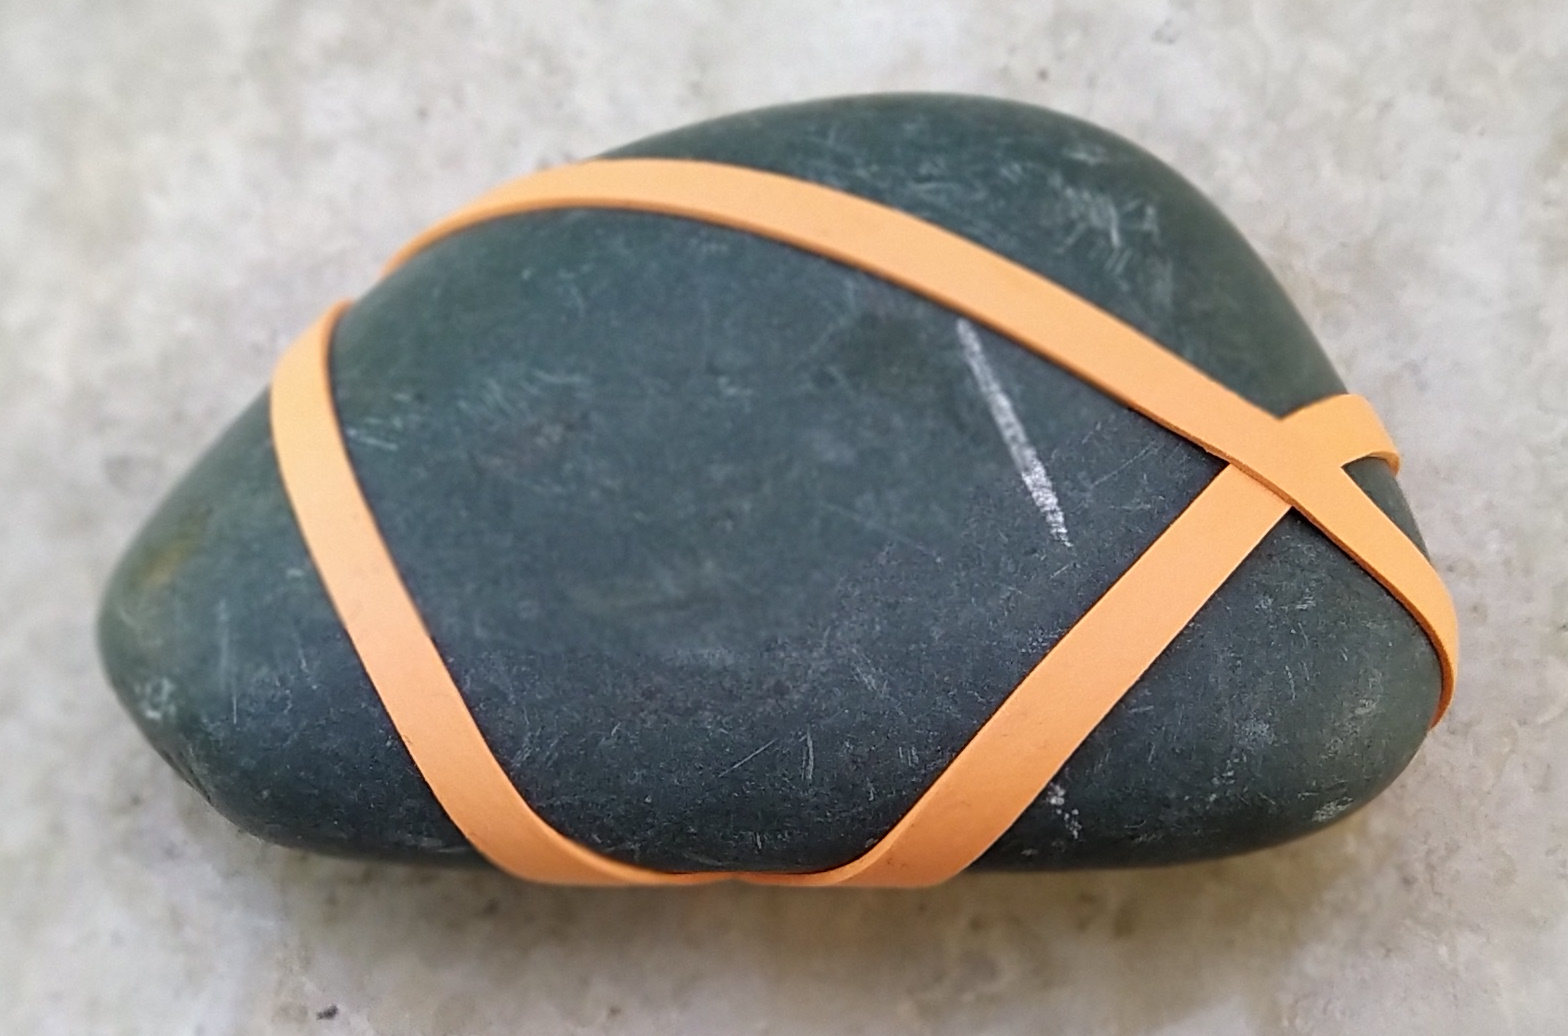
\includegraphics[width=\textwidth]{pics/pebble.jpg}
\end{minipage}\hfill
\begin{minipage}{.34\textwidth}
\centering
\includegraphics{mppics/pic-50}
\end{minipage}
\end{figure}
The combinatorics of self-crossings can be described by a closed plane curve --- it is the curve that the rubber band follows in a plane parametrization of the surface with one point removed.
For example, if you could turn the pebble around you would see that self-crossings of the rubber band on the picture can be described by the plane curves on the right diagram.

We assume that the pebble has stongly convex smooth frictionless boundary;
so the rubber band models a closed geodesic on a smooth strongly convex surface.
Suppose that we are interested in possible patterns of self-crossings; more precicely, the following question:

\medskip

\emph{What are the possible combinatoric types of self-crossings of closed geodesic on a strongly convex smooth closed surface?}

\medskip

It is a good exercise --- it could be explained to anyone, but if a motivated student starts to think about it, then he will have to rediscover  a considerable part of the differential geometry of surfaces.

\begin{figure}[ht!]
\begin{center}
\includegraphics{mppics/pic-55}
\end{center}
\end{figure}

We will discuss \emph{forbidden} configurations with 3 double self-crossings;
that is, configurations that cannot appear for closed geodesic of a strongly convex closed surface. 
Among all the possible 6 patterns shown on the diagram,
only two --- no 5 and 6 are forbidden.
Showing the possibility of configurations 1--4 requires some ingenuity,
but, the forbidden examples make mathematicians happier.

(Mathematicians like to forbid, is not it strange?)

The reader is welcome to try other cases, but the general question seems to be hard;
we do not expect to see a complete classification in our lifetime.

In what follows, we briefly discuss Gauss--Bonnet formula and Alexandrov--Toponogov theorem and apply them to forbid configurations 5 and 6.
These theorems are discussed in our textbook \cite{petrunin-zamora} which we like, but there plenty other resources.

\section*{Gauss--Bonnet and no 5}

Further we assume that $\Sigma$ is a closed strongly convex surface;
in particular, $\Sigma$ is homeomorphic to the sphere and has strictly positive Gauss curvature.

Suppose that $\Delta$ is an $n$-gon on $\Sigma$ with geodesic sides.
From the \emph{Gauss--Bonnet formula} it follows that the sum of the internal angles of $\Delta$ cannot be smaller than $(n\z-2)\cdot\pi$.
In particular, if $\Delta$ is a triangle with angles $\alpha$, $\beta$, and $\gamma$, then
\[\alpha+\beta+\gamma>\pi.\leqno({*})\]
Also the Gauss--Bonnet formula implies that the integral of Gauss curvature along the whole $\Sigma$ is exactly $4\cdot\pi$.

\begin{wrapfigure}{r}{40 mm}
\vskip-0mm
\centering
\includegraphics{mppics/pic-3}
\end{wrapfigure}

\parit{Let us show that configuration no 5 is forbidden.}
Suppose there is a geodesic with self-crossings as on the diagram;
it divides the surface $\Sigma$ into one triangle, say $\Delta$, one hexagon, and three monogons.
Denote by $\alpha$, $\beta$, and $\gamma$ the internal angles of $\Delta$.

Note that three monogons have internal angles $\alpha$, $\beta$, and $\gamma$ respectively.
By Gauss--Bonnet formula, the integral of Gauss curvature along each monogon is $\pi+\alpha$, $\pi+\beta$, and $\pi+\gamma$ respectively.
By $({*})$ the integral of Gauss curvature along the three monogons $\Sigma$ exceeds $4\cdot \pi$.
But $4\cdot \pi$ is the integral of Gauss curvature along the \emph{whole} $\Sigma$  --- a contradiction.

\section*{Alexandrov--Toponogov and no 6}

Let $\Delta$ be a geodesic triangle with angles $\alpha$, $\beta$, and $\gamma$ on the surface $\Sigma$.
Assume that the sides of $\Delta$ are length minimizing geodesics among the curves in $\Delta$ with the same endpoints, then the inequality $({*})$ can be made more exact.

Namely consider the so-called \emph{model triangle} $\tilde\Delta$ of $\Delta$; that is, $\tilde\Delta$ is a plane triangle with equal corresponding sides.
Since the sides are length-minimizing, they satisfy the triangle inequality; therefore the model triangle is defined.

Denote by $\tilde \alpha$, $\tilde \beta$ and $\tilde \gamma$ the angles of $\tilde\Delta$ respectively.
Then 
\[
\alpha> \tilde \alpha,
\qquad
\beta> \tilde \beta,
\qquad
\text{and}
\qquad
\gamma> \tilde \gamma.
\leqno({*}{*})
\]
Since $\tilde\alpha+\tilde\beta+\tilde\gamma=\pi$, this inequality implies $({*})$.

The inequality $({*}{*})$ easily follows from the proof of the \emph{Alexandrov--Toponogov comparison theorem}.
We leave it as an exercise to those who know this proof;
the rest of the readers could simply believe that it is true.

\begin{figure}[!ht]
\begin{minipage}{.38\textwidth}
\centering
\includegraphics{mppics/pic-472}
\end{minipage}\hfill
\begin{minipage}{.58\textwidth}
\centering
\includegraphics{mppics/pic-473}
\end{minipage}
\end{figure}

\parit{Let us show that configuration no 6 is forbidden.}
Arguing by contradiction, suppose that $\Sigma$ contains such a geodesic $\gamma$;
assume that arcs and angles are labeled as on the left diagram.

Applying the Gauss--Bonnet formula to the quadrangle and pentagon that the geodesic cuts from $\Sigma$, we get that
\[2\cdot\alpha<\beta+\gamma
\qquad\text{and} \qquad
2\cdot\beta+2\cdot \gamma<\pi+\alpha.\leqno(\asterism)\]
It follows that $\alpha <\tfrac \pi 3$.


Consider the part of $\gamma$ without the arc~$a$.
It cuts from $\Sigma$ a pentagon $\Delta$ with sides and angles shown on the diagram on the right.

\begin{wrapfigure}{r}{50 mm}
\vskip-0mm
\centering
\includegraphics{mppics/pic-474}
\end{wrapfigure}

Let us add additional vertices on the sides of $\Delta$ so that each side becomes length-minimizing.
Choose a vertex $v$ and subdivide $\Delta$ into triangles with minimizing sides by joining $v$ to other vertices.

Consider a model triangle for each triangle in the subdivision;
the model triangles lie in the plane and we suppose that they share sides as in $\Delta$.
By the comparison inequality $({*}{*})$, the angles of the model triangles do not exceed the corresponding angles of the original triangle.
Therefore the model triangles form a convex plane polygon $\tilde\Delta$.
Moreover, the five angles of $\tilde\Delta$ that correspond to angles of $\Delta$ do not exceed those.

\begin{wrapfigure}{r}{50 mm}
\vskip-2mm
\centering
\includegraphics{mppics/pic-500}
\vskip0mm
\end{wrapfigure}

It remains to show that the described plane polygon $\tilde\Delta$ does not exist.
Let us orient its  sides counterclockwise;
denote the obtained vectors by $s_1,\dots,s_k$.

On one hand, the conditions on the angles of polygons imply that the vectors $s_i$ point in the complement of white sectors shown with angles marked on the diagram.
The sum of magnitudes of the vectors in each black sector is also marked.
Let $v$, $v'$, $w$, $w'$ be the marked unit vectors;
set $r=v+v'+w+w'$.
Observe that $(\asterism)$ implies that $r\ne 0$,
and, moreover, 
\[\langle r,s_1\rangle+\dots+\langle r,s_k\rangle>0.\]
On the other hand, we have $s_1+\dots+s_k=0$ --- a contradiction.




{\sloppy
\printbibliography[heading=bibintoc]
\fussy
}

\end{document}
